\documentclass[11pt]{article}

\usepackage[utf8]{inputenc}
\usepackage{amsmath,amssymb,amsthm}
\usepackage{graphicx}
\usepackage{hyperref}
\usepackage{float}
\usepackage{geometry}

\geometry{
  a4paper,
  left=25mm,
  right=25mm,
  top=25mm,
  bottom=25mm
}

\title{\textbf{A Unified Framework for Distributed Quantum Databases\\
\vspace{0.5cm}
\large Integrating Topos-Theoretic Approaches, Entanglement, and QEC Pipelines}}
\author{Matthew Long \\
\small Magneton Labs}
\date{\today}

\begin{document}

\maketitle

\begin{abstract}
In this paper, we present an integrated framework for designing and analyzing distributed quantum databases (DQDB). We merge three distinct perspectives: (1) a topos-theoretic construction that ensures global consistency via entanglement; (2) a structured approach to quantum database theory that accounts for concurrency and non-local correlations; and (3) a quantum error correction (QEC) pipeline that maintains data fidelity throughout the system. By combining these viewpoints, we propose a novel architecture for constructing robust, scalable, and semantically rich quantum databases capable of distributed operation. This unification allows us to expand on both the theoretical underpinnings and the practical designs of quantum databases, highlighting how entanglement and logical error correction techniques jointly ensure a coherent global state and resilience against noise. Our hope is that these unified methods serve as a cornerstone for future quantum data management systems, facilitating reliable communication, efficient query processing, and guaranteed consistency across geographically separated nodes.
\end{abstract}

\section{Introduction}
Classical distributed databases and the management of data in geographically separated sites have formed the basis of large-scale applications in finance, scientific computing, and enterprise software. As quantum computing continues to advance, there is a growing need to adapt and extend these distributed paradigms to the quantum realm \cite{nielsen_chuang, verstraete_review}. A distributed quantum database (DQDB) aims to store and manage quantum information across multiple nodes in a way that maintains consistency, coherence, and security.

While the core principles of database theory (e.g., concurrency control, replication, transaction management) remain relevant, the quantum setting adds new complexities: non-classical correlations (entanglement), quantum error correction needs, and the possibility of topological or category-theoretic frameworks (such as topos theory) to track logical consistency \cite{abramsky, heunen}. Entanglement can serve as a powerful tool for synchronization, while quantum error correction (QEC) offers a crucial mechanism for ensuring data fidelity in noisy quantum channels or hardware. 

In this paper, we take three previously developed approaches:
\begin{enumerate}
    \item A \textbf{topos-theoretic approach} to quantum databases, focusing on the use of sheaves, presheaves, and other categorical tools to model global consistency in the presence of local quantum subsystems.
    \item A \textbf{quantum database theory} framework that highlights concurrency, entanglement-based transactions, and non-local correlations for data queries and updates.
    \item A \textbf{quantum error correction pipeline} for systematically constructing fault-tolerant operations and logical qubits that ensure robust storage and retrieval in the presence of noise.
\end{enumerate}
We integrate these perspectives into one cohesive framework, highlighting:
\begin{itemize}
    \item How a topos-theoretic perspective naturally incorporates entanglement to guarantee coherence and consistency across multiple nodes.
    \item How concurrency control and data-level operations in a quantum setting can exploit entanglement, measurement, and multi-node quantum channels.
    \item How error-correction pipelines fit into the architecture, allowing for distributed quantum states to remain fault-tolerant through repeated or adaptive error-correcting steps.
\end{itemize}

By merging these viewpoints, we propose a new generation of distributed quantum databases that seamlessly unify theoretical depth (topos models), system-level design (entanglement-based concurrency), and implementation-level resilience (quantum error correction). We aim for an end result that is logically consistent, robust against noise, and scalable to large numbers of nodes.

\subsection{Paper Organization}
The paper is organized as follows:
\begin{itemize}
    \item Section~\ref{sec:background} provides a survey of the relevant topics, including a brief overview of classical distributed databases, quantum database paradigms, topos theory, and quantum error correction.
    \item Section~\ref{sec:topos_theory} describes our topos-theoretic approach to modeling distributed quantum information, including sheaf-based approaches to local-global consistency and the role of entanglement.
    \item Section~\ref{sec:qdb_theory} outlines how concurrency control, transactions, and queries extend into the quantum realm, using entanglement for synchronization and measuring correctness.
    \item Section~\ref{sec:qec_pipeline} details the quantum error correction pipeline as integrated into the distributed architecture, emphasizing the synergy between entanglement distribution, error correction, and data integrity.
    \item Section~\ref{sec:unified_architecture} presents our unified framework, describing the architectural layers, protocols, and interactions among the topos model, quantum transaction logic, and QEC pipeline components.
    \item Section~\ref{sec:implementation} discusses possible implementation strategies and hardware considerations, including quantum networking and specialized qubit technologies.
    \item Section~\ref{sec:future_work} outlines directions for future research, including advanced concurrency models, topological quantum error-correcting codes, and expansions of the topos approach to more general categorical frameworks.
    \item Section~\ref{sec:conclusion} concludes the paper.
\end{itemize}

\section{Background and Related Work}
\label{sec:background}

\subsection{Classical Distributed Databases}
Classical distributed databases rely on strategies like sharding, replication, and partitioning to scale to large numbers of nodes. Concurrency control mechanisms such as two-phase commit (2PC) and distributed transaction protocols guarantee \emph{atomicity}, \emph{consistency}, \emph{isolation}, and \emph{durability} (ACID properties). Consensus protocols like Paxos or Raft maintain replicated logs that ensure consistency across distributed sites \cite{gray_transaction, lamport_paxos}.

While these techniques work for classical data (bits stored in conventional memory), quantum data poses unique challenges. For instance, qubits cannot be cloned due to the no-cloning theorem; entanglement cannot be straightforwardly replicated; and measurements collapse the quantum state, irreversibly extracting classical information \cite{preskill}. Therefore, standard concurrency, replication, and consistency protocols must be adapted or rethought in the quantum setting.

\subsection{Quantum Database Paradigms}
Quantum databases have been proposed in various contexts. Some efforts focus on \emph{quantum query complexity}, using the quantum advantage in searching unsorted databases \cite{grover}. Others focus on \emph{quantum-safe cryptography}, ensuring database queries cannot be compromised by quantum adversaries. More recently, \emph{quantum database management systems} (QDBMS) attempt to create systems that store and manipulate qubits \textit{themselves}, not just classical data. These QDBMS solutions address issues of how to physically store quantum states, track entanglement or correlation structure, and facilitate quantum transactions \cite{lloyd, giovannetti}.

\subsection{Topos Theory and Quantum Structures}
\label{sec:topos_background}
Topos theory generalizes set theory using category-theoretic tools, providing a powerful language to discuss local and global structures in a unified manner \cite{maclane, johnstone, bell}. In the context of quantum mechanics, \emph{presheaf topos} or \emph{sheaf topos} can model the localization of measurement outcomes and contextual variables, capturing non-commuting observables in an “almost classical” local sense \cite{isham_topos, doering_isham}.

When extended to distributed quantum systems, the topos perspective helps define how local data patches (localized quantum states at each node) can be glued together to form a consistent global state---or a “global section” in topos parlance. Entanglement plays a critical role here, representing correlations that cannot be captured by purely classical sheaf structures.

\subsection{Quantum Error Correction (QEC)}
Quantum error correction (QEC) is vital for preserving quantum states against decoherence, gate errors, and other noise sources \cite{shor, steane, nielsen_chuang}. Common QEC protocols (e.g., Steane code, Shor code, surface codes) allow one to store logical qubits in multiple physical qubits, detecting and correcting a bounded number of errors. In a distributed scenario, nodes must coordinate QEC procedures, sometimes requiring entangling operations across network links \cite{jiang, wallraff_review}.

\begin{figure}[H]
    \centering
    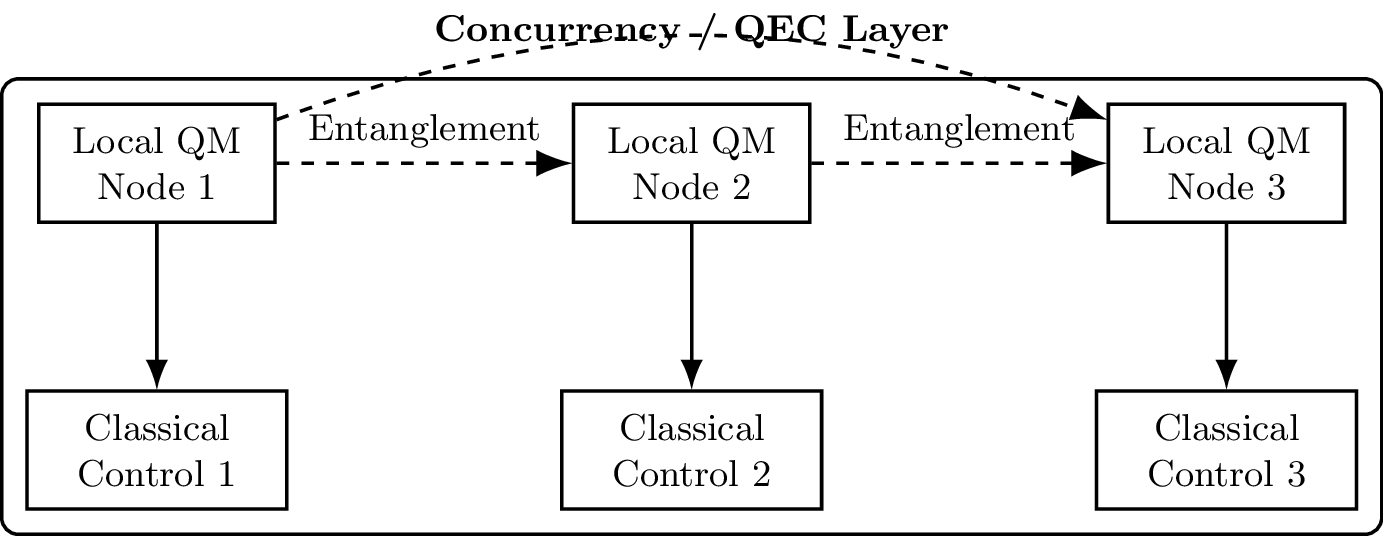
\includegraphics[width=0.6\textwidth]{dist_qdb_arch_fig.png}
    \caption{A high-level representation of a distributed quantum database architecture, showing local quantum memories, classical control nodes, entanglement channels (dashed lines), and an overarching concurrency/QEC layer.}
    \label{fig:dqdb_architecture}
\end{figure}

By combining topological or concatenated QEC codes with entanglement-based resource sharing, a distributed system can maintain a robust, global quantum state. Achieving efficient error correction is thus crucial for realistic quantum database operations.

\section{A Topos-Theoretic Approach to Distributed Quantum Databases}
\label{sec:topos_theory}
Topos theory offers a unified foundation that can describe both “classical-like” local operations and “global” quantum phenomena, particularly entanglement. In this section, we build from prior work on applying presheaf-based constructions to quantum measurement scenarios and extend them to the distributed case.

\subsection{Sheaves, Presheaves, and Local Contexts}
A key premise in topos-based quantum models is that each \emph{context} or \emph{chart} describes a subset of commuting observables or a partial set of measurement outcomes \cite{isham_topos, doering_isham}. By gluing these contexts together under suitable compatibility conditions, we obtain a global description that is more subtle than simply combining classical states, due to potential entanglement.

For a distributed quantum database, each node $N_i$ has:
\begin{itemize}
    \item A local Hilbert space $\mathcal{H}_i$.
    \item A set of commuting measurement operators $\{M_{i,\alpha}\}$ relevant to local data queries.
    \item A set of local contexts $C_{i}$, each describing a partial subalgebra of $\mathcal{H}_i$.
\end{itemize}
We form a \emph{global} presheaf or sheaf by specifying how these local contexts morph into a shared global context. Entanglement can appear as a mismatch between purely local classical assignments; it is precisely the phenomenon that requires a more sophisticated global object than set-theoretic gluing.

\subsection{Entanglement as a Gluing Constraint}
In classical sheaf theory, we require local sections to agree on overlaps. In quantum topos terms, local sections must be consistent with respect to partial trace operations or partial measurement outcomes in areas of overlap. Entanglement constraints appear as conditions that link the states of different nodes, requiring certain correlations in measurement outcomes.

For example, suppose we have a bipartite system between nodes $N_1$ and $N_2$. If $N_1$ measures an observable $M_1$ and obtains a result $m_1$, the topos approach ensures that the restriction of the global section to $N_2$’s local context is consistent with the entangled global state. This leads to the phenomenon that $N_2$'s measurement distribution might update instantly as part of the global wavefunction collapse (from the perspective of the entire system), yet no faster-than-light communication of classical information occurs \cite{bruza, redei}.

\subsection{Categorical View of Transactions}
Transactions in a quantum sense can be described as morphisms that carry local contexts to new states or contexts, subject to concurrency rules. A transaction that updates local data in node $N_i$ can be seen as a morphism in the topos from one presheaf section to another. Entanglement correlations might restrict which transactions are allowed or how they can be composed. This perspective lays the groundwork for concurrency control in a quantum database: rather than two-phase locking, we might adopt \emph{two-phase entanglement distribution} or \emph{multi-phase measurement scheduling} that ensures consistency without directly copying data \cite{abramsky, heunen}.

\begin{figure}[H]
    \centering
    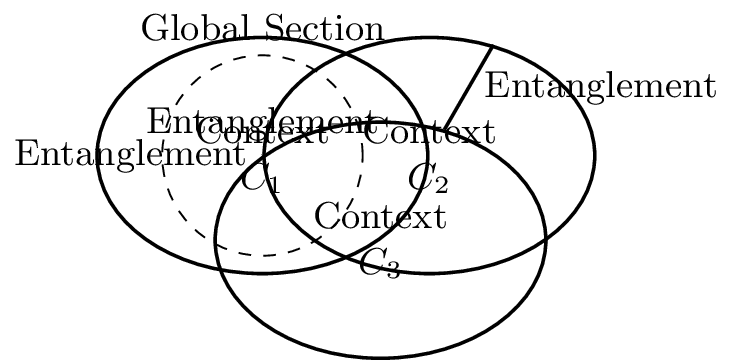
\includegraphics[width=0.55\textwidth]{topos_entanglement_fig.png}
    \caption{Schematic of how local presheaves (contexts) in a quantum database can be glued into a global section. Entanglement imposes non-trivial constraints on the global consistency conditions.}
    \label{fig:topos_gluing}
\end{figure}

\section{Quantum Database Theory: Entanglement, Concurrency, and Transactions}
\label{sec:qdb_theory}
Where classical concurrency control ensures ACID properties in distributed databases, quantum concurrency must account for the possibility that multiple transactions share entangled resources. Moreover, measurement events cause fundamental changes in the quantum system.

\subsection{Entanglement-Based Concurrency and Locking}
In classical systems, locks isolate conflicting transactions until they can be safely committed. In a quantum system, because qubits cannot be “read” without measurement (leading to wavefunction collapse), concurrency is better managed by:

\begin{enumerate}
    \item \textbf{Entanglement scheduling}: Decide how entanglement is distributed among transactions to minimize destructive interference.
    \item \textbf{Measurement ordering}: Carefully order or group measurement operations if multiple transactions might measure correlated qubits. 
    \item \textbf{Classical side-channel for commit protocols}: Although quantum data cannot be cloned, classical bits can still be used to coordinate commit or rollback decisions after partial measurement results.
\end{enumerate}

This concurrency control prevents non-commuting operations from interfering with each other in destructive ways, while maintaining enough data about outcomes to preserve consistency.

\subsection{Global Consistency via Entangled States}
Unlike classical replication, quantum “replication” (if any) occurs via entanglement. For instance, in a GHZ state distributed across three nodes, measuring one qubit in the computational basis can instantly define constraints on the other two qubits. This non-local effect can be leveraged for global consistency checks, but must be carefully orchestrated so as not to collapse the entire distributed state prematurely.

\subsection{Transaction Lifecycle}
Figure \ref{fig:qdb_transaction_flow} illustrates a typical transaction in a distributed quantum database:

\begin{figure}[H]
    \centering
    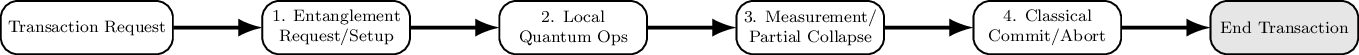
\includegraphics[width=0.65\textwidth]{qdb_trans_flow_fig.png}
    \caption{Sample quantum transaction lifecycle showing entanglement distribution, local operations, partial measurements, classical commit phase, and final consolidation of quantum states.}
    \label{fig:qdb_transaction_flow}
\end{figure}

\begin{enumerate}
    \item \textbf{Entanglement request}: The transaction requests entangled pairs/qubits to share across relevant nodes.
    \item \textbf{Local quantum operations}: Each node performs local gates or unitaries on its portion of the entangled state.
    \item \textbf{Measurement or partial collapse}: Some qubits are measured to extract classical data or to finalize the transaction’s effect on the database.
    \item \textbf{Classical commit/abort}: Based on the measurement outcomes, classical logic decides whether to \emph{commit} (apply) or \emph{abort} (revert) the changes, possibly requiring an additional entanglement re-initialization step if the transaction fails.
\end{enumerate}

This design ensures the physically distributed quantum states remain consistent, while still allowing concurrency in the form of parallel entanglement usage among different transactions (provided they act on disjoint sets of qubits or utilize commuting operations).

\section{Quantum Error Correction Pipeline}
\label{sec:qec_pipeline}
Our integrated framework must incorporate a \emph{quantum error correction pipeline} (QEC pipeline) that ensures data fidelity across distributed nodes. Quantum errors occur due to decoherence, gate imperfections, environmental noise, etc. The QEC pipeline introduced in prior work includes the following stages:

\begin{enumerate}
    \item \textbf{Physical Qubit Encoding}: Map each logical qubit or qudit into a block of physical qubits using a chosen error-correcting code (e.g., surface code, Shor code, Steane code).
    \item \textbf{Syndrome Measurement}: Periodically measure stabilizers or other check operators to detect potential errors.
    \item \textbf{Syndrome Processing and Correction}: Classically process the syndrome measurements to infer likely errors and apply corrective unitary operations.
    \item \textbf{State Verification/Calibration}: Optionally verify that the corrected state meets fidelity thresholds. If not, trigger further protocols, such as entanglement distillation or partial re-encoding.
    \item \textbf{Entanglement Renewal}: In a distributed system, some QEC protocols require re-establishing or refreshing entangled resource states (e.g., Bell pairs or GHZ states) used for teleportation-based gates or distributed logical operations.
\end{enumerate}

\begin{figure}[H]
    \centering
    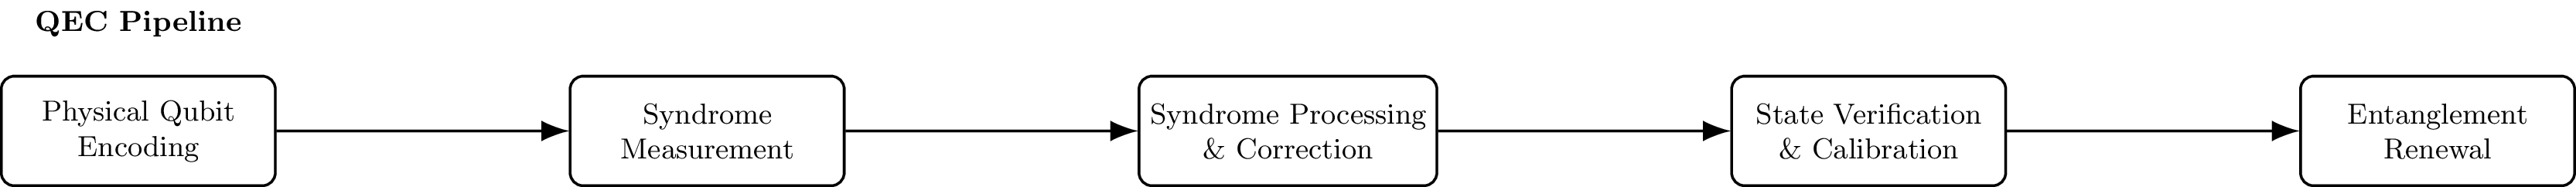
\includegraphics[width=0.7\textwidth]{qec_pipeline_fig.png}
    \caption{Overview of a generic quantum error correction pipeline in a distributed setting. Logical qubits are encoded in multiple physical qubits across multiple nodes, with periodic syndrome measurements and corrective steps.}
    \label{fig:qec_pipeline}
\end{figure}

In a distributed quantum database, these QEC steps must integrate seamlessly into the transaction protocols. For instance, before committing a transaction that modifies a logical qubit, the system may force a QEC cycle to ensure that the state is still valid. Likewise, concurrency control layers must be mindful of QEC procedures that may temporarily occupy certain qubits or require multi-node synchronization \cite{fowler, campbell}.

\subsection{Interaction with Entanglement Distribution}
Many QEC protocols rely on entangled resource states, such as Bell pairs used in teleportation-based gates or parity checks. In a distributed database, these resource states need to be shared across nodes. The pipeline must manage not only the local error correction of each block but also the \emph{global} correction of entangled states spanning multiple nodes. This may involve entanglement distillation protocols, where raw entanglement is refined into high-fidelity Bell or GHZ states \cite{bennett, pan_distillation}.

\subsection{Scalability and Overheads}
A critical concern is overhead in the number of physical qubits, classical communication channels, and syndrome processing. In large-scale quantum databases, naive QEC with high-distance codes might become impractical, so hierarchical or adaptive approaches could become more attractive \cite{lidar_brun}. Careful scheduling must balance the demands of transaction concurrency, QEC cycles, and data queries in a dynamic environment where nodes may come online or offline.

\section{A Unified Architecture for Distributed Quantum Databases}
\label{sec:unified_architecture}
Bringing together the topos-theoretic viewpoint, the quantum database concurrency model, and the QEC pipeline, we propose a unified architecture that can be outlined in the following layers:
\begin{enumerate}
    \item \textbf{Physical Layer}: Real qubits in superconducting circuits, ion traps, photonic systems, or other quantum hardware. Physical qubits are arranged locally at each node, with quantum networking channels (fiber or free-space) enabling entanglement distribution.
    \item \textbf{Error Correction and Entanglement Management Layer}: A specialized layer that handles the encoding of logical qubits, distribution and distillation of entangled pairs, and periodic QEC cycles. This layer also provides interfaces for concurrency control to “reserve” certain qubits during a transaction or to schedule syndrome measurements.
    \item \textbf{Topos-Theoretic Consistency Layer}: Using the concepts from Section~\ref{sec:topos_theory}, this layer maintains a global presheaf/sheaf structure that tracks local measurement contexts and gluing conditions. It interprets entanglement as constraints, thereby allowing a higher-level logic to coordinate partial measurements and global sections. 
    \item \textbf{Quantum Transaction Management Layer}: The system component that receives transaction requests (queries, updates, etc.). It is responsible for:
    \begin{itemize}
        \item Allocating entangled resource states to the requesting transaction.
        \item Orchestrating local quantum operations and measurements.
        \item Coordinating with the Error Correction and Entanglement Management Layer to ensure fidelity remains above threshold.
        \item Committing or aborting transactions based on measurement outcomes and classical agreement.
    \end{itemize}
    \item \textbf{Application Layer}: Classical or hybrid quantum-classical applications that issue queries or analytics tasks (e.g., quantum machine learning workflows, large-scale optimization queries). This layer sees a “logical” database interface, abstracted from the complexities of QEC or topos-based consistency.
\end{enumerate}

\section{Implementation Considerations}
\label{sec:implementation}
Although largely theoretical, prototypes of distributed quantum computers are emerging \cite{kimble_quantum_internet}, making partial implementations of a distributed quantum database more realistic. 

\subsection{Hardware Platforms}
Potential hardware candidates include:
\begin{itemize}
    \item \emph{Trapped Ions}: Well-developed qubit coherence times, relatively straightforward entanglement generation, though network scaling is non-trivial \cite{blatt_wineland}.
    \item \emph{Superconducting Circuits}: Rapid gate speeds, active research in quantum networking with microwave-to-optical conversion, but short coherence times may complicate distributed protocols \cite{kjaergaard_review}.
    \item \emph{Photonic Systems}: Natural for distributing entanglement across nodes via optical fibers or free-space. However, deterministic gates on photonic qubits remain challenging \cite{kok_photonic}.
\end{itemize}

Implementers must consider the trade-offs between gate fidelity, connectivity, network entanglement bandwidth, and the overhead of error correction.

\subsection{Network Protocols and Entanglement Distribution}
At the networking level, the system must establish quantum links between nodes. Protocols like \emph{entanglement swapping}, \emph{quantum teleportation}, or \emph{repeaters} can extend these links over large distances \cite{briegel_repeater, munro_repeater}. Realistic implementations also require \emph{heralding} signals to confirm successful entanglement, plus classical side-channels for synchronization.

\subsection{Software Stack and Control}
A layered software stack might include:
\begin{enumerate}
    \item A low-level hardware control interface (pulses, gate instructions).
    \item An \emph{error correction runtime} that implements syndrome measurement schedules, decoders (e.g., minimum-weight matching for surface codes \cite{fowler}), and qubit assignment.
    \item A \emph{transaction manager} that can invoke entanglement distribution, track partial measurement results, and coordinate concurrency among multiple queries.
    \item A \emph{topos-based logic engine} that maintains an internal representation of the global presheaf structure and ensures that local contexts remain consistent with the global constraints.
    \item High-level \emph{APIs} for quantum applications to issue queries or define new stored quantum states.
\end{enumerate}

\section{Future Directions}
\label{sec:future_work}
Several open problems and research directions emerge from this unified framework:

\begin{itemize}
    \item \textbf{Topological Codes and Sheaf Theory}: Investigate deeper connections between topological QEC (e.g., surface codes) and topos theory. Both revolve around local patching conditions and global consistency; synergy might provide new insights into error-resilient \emph{and} logically consistent distributed states.
    \item \textbf{Alternative Categorical Approaches}: Beyond topos theory, other category-theoretic frameworks (e.g., monoidal categories, enriched categories) could further refine concurrency or composition aspects of quantum transactions.
    \item \textbf{Advanced Concurrency Control}: Develop protocols for \emph{optimistic concurrency}, \emph{multi-version concurrency}, or \emph{snapshot isolation} in quantum contexts, possibly leveraging partial measurement or approximate subspaces.
    \item \textbf{Post-Quantum Cryptography Integration}: Although not the core of this framework, ensuring that the classical channels remain secure in the presence of quantum adversaries is crucial. Merging quantum-safe cryptographic routines into the transaction management or QEC pipeline could bolster overall security.
    \item \textbf{Resource Estimation}: A major practical question is the overhead in terms of qubit counts, entanglement distribution rates, classical communication, and latency. Detailed resource estimation and simulation can guide feasible near-term prototypes.
    \item \textbf{Hybrid Classical-Quantum Queries}: Real-world applications may mix classical data with quantum states. Extending classical database technology (e.g., SQL, NoSQL) with quantum operators and ensuring the entire system remains consistent is a multi-layer challenge.
\end{itemize}

\section{Conclusion}
\label{sec:conclusion}
Distributed quantum databases offer a tantalizing vision of storing and managing quantum data across geographically separated nodes. By unifying three distinct perspectives---topos-theoretic modeling for global consistency, entanglement-centric concurrency control for transactions, and a robust quantum error correction pipeline---we have proposed an integrated framework that addresses both theoretical coherence and practical resilience.

Topos theory provides a mathematical language to describe local contexts and global sections in the presence of non-classical correlations. The concurrency model adapted for quantum data handles measurement-induced collapse, entanglement distribution, and classical commit protocols. Meanwhile, quantum error correction ensures that, despite noisy hardware and decoherence, logical qubits and global entangled states remain robust enough to support queries and updates.

While considerable challenges remain, particularly in hardware development, resource overhead, and the design of efficient concurrency protocols, this merged framework serves as a blueprint for future research and prototyping. As quantum hardware matures, the ideas outlined here could inform the creation of truly distributed quantum information systems, enabling powerful data-driven quantum computing applications that surpass classical limits.

\bigskip

\begin{thebibliography}{99}
\bibitem{nielsen_chuang} M. A. Nielsen and I. L. Chuang, \emph{Quantum Computation and Quantum Information}, 10th Anniversary Edition, Cambridge University Press, 2010.

\bibitem{verstraete_review} F. Verstraete, J. I. Cirac, and V. Murg, ``Matrix Product States, Projected Entangled Pair States, and Variational Renormalization Group Methods for Quantum Spin Systems,'' \emph{Advances in Physics}, 57(2), 143–224 (2008).

\bibitem{abramsky} S. Abramsky and B. Coecke, ``Categorical Quantum Mechanics,'' in \emph{Handbook of Quantum Logic and Quantum Structures} (eds. K. Engesser, D. M. Gabbay, D. Lehmann), Elsevier, 2009.

\bibitem{heunen} C. Heunen, \emph{Categorical Quantum Models and Logics}, Oxford University Press, 2019.

\bibitem{gray_transaction} J. Gray, ``Notes on Data Base Operating Systems,'' in \emph{Operating Systems: An Advanced Course}, pp. 393–481, Springer, 1978.

\bibitem{lamport_paxos} L. Lamport, ``The Part-Time Parliament,'' \emph{ACM Transactions on Computer Systems}, 16(2), 133–169 (1998).

\bibitem{preskill} J. Preskill, ``Quantum Computing in the NISQ era and beyond,'' \emph{Quantum}, 2, 79 (2018).

\bibitem{grover} L. K. Grover, ``A Fast Quantum Mechanical Algorithm for Database Search,'' in \emph{Proceedings of the 28th Annual ACM Symposium on the Theory of Computing} (STOC), pp. 212–219 (1996).

\bibitem{lloyd} S. Lloyd, M. Mohseni, and P. Rebentrost, ``Quantum Algorithms for Supervised and Unsupervised Machine Learning,'' \emph{arXiv:1307.0411} (2013).

\bibitem{giovannetti} V. Giovannetti, S. Lloyd, and L. Maccone, ``Quantum Random Access Memory,'' \emph{Physical Review Letters}, 100, 160501 (2008).

\bibitem{maclane} S. Mac Lane, \emph{Categories for the Working Mathematician}, Springer, 2nd ed., 1998.

\bibitem{johnstone} P. T. Johnstone, \emph{Sketches of an Elephant: A Topos Theory Compendium}, Oxford University Press, 2002.

\bibitem{bell} J. L. Bell, \emph{Toposes and Local Set Theories}, Dover, 2008.

\bibitem{isham_topos} C. J. Isham, ``Topos Methods in the Foundations of Physics,'' in \emph{Deep Beauty: Understanding the Quantum World Through Mathematical Innovation}, 2011.

\bibitem{doering_isham} A. D\"oring and C. J. Isham, ``A Topos Foundation for Theories of Physics: I-V,'' \emph{Journal of Mathematical Physics}, 49, 053515 (2008).

\bibitem{bruza} P. D. Bruza, Z. Wang, and B. B. Kitto, ``Quantum Cognition: A New Theoretical Approach to Psychology,'' \emph{Trends in Cognitive Sciences}, 15(8), 383–393 (2012).

\bibitem{redei} M. R\'edei and S. J. Summers, ``Local Quantum Probability,'' \emph{Reports on Mathematical Physics}, 53(2), 317–348 (2004).

\bibitem{shor} P. W. Shor, ``Scheme for Reducing Decoherence in Quantum Computer Memory,'' \emph{Physical Review A}, 52, R2493 (1995).

\bibitem{steane} A. M. Steane, ``Error Correcting Codes in Quantum Theory,'' \emph{Physical Review Letters}, 77, 793 (1996).

\bibitem{jiang} L. Jiang \emph{et al.}, ``Distributed Quantum Computation Based on Small Quantum Registers,'' \emph{Physical Review A}, 79, 032325 (2009).

\bibitem{wallraff_review} A. Wallraff \emph{et al.}, ``Approaching Unit Visibility for Control of a Superconducting Qubit with Dispersive Readout,'' \emph{Physical Review Letters}, 95, 060501 (2005).

\bibitem{fowler} A. G. Fowler, M. Mariantoni, J. M. Martinis, and A. N. Cleland, ``Surface Codes: Towards Practical Large-Scale Quantum Computation,'' \emph{Physical Review A}, 86, 032324 (2012).

\bibitem{campbell} E. T. Campbell, B. M. Terhal, and C. Vuillot, ``Roads Towards Fault-Tolerant Universal Quantum Computation,'' \emph{Nature}, 549, 172–179 (2017).

\bibitem{bennett} C. H. Bennett, G. Brassard, S. Popescu, B. Schumacher, J. A. Smolin, and W. K. Wootters, ``Purification of Noisy Entanglement and Faithful Teleportation via Noisy Channels,'' \emph{Physical Review Letters}, 76, 722 (1996).

\bibitem{pan_distillation} J.-W. Pan, C. Simon, \v{C}. Brukner, and A. Zeilinger, ``Entanglement Purification for Quantum Communication,'' \emph{Nature}, 410, 1067–1070 (2001).

\bibitem{lidar_brun} D. A. Lidar and T. A. Brun, \emph{Quantum Error Correction}, Cambridge University Press, 2013.

\bibitem{kimble_quantum_internet} H. J. Kimble, ``The Quantum Internet,'' \emph{Nature}, 453, 1023–1030 (2008).

\bibitem{blatt_wineland} R. Blatt and D. Wineland, ``Entangled States of Trapped Atomic Ions,'' \emph{Nature}, 453, 1008–1015 (2008).

\bibitem{kjaergaard_review} M. Kjaergaard \emph{et al.}, ``Superconducting Qubits: Current State of Play,'' \emph{Annual Review of Condensed Matter Physics}, 11, 369–395 (2020).

\bibitem{kok_photonic} P. Kok \emph{et al.}, ``Linear Optical Quantum Computing with Photonic Qubits,'' \emph{Reviews of Modern Physics}, 79, 135 (2007).

\bibitem{briegel_repeater} H.-J. Briegel, W. D\"ur, J. I. Cirac, and P. Zoller, ``Quantum Repeaters: The Role of Imperfect Local Operations in Quantum Communication,'' \emph{Physical Review Letters}, 81(26), 5932–5935 (1998).

\bibitem{munro_repeater} W. J. Munro, A. M. Stephens, S. J. Devitt, K. A. Harrison, and K. Nemoto, ``Quantum Communication Without the Necessity of Quantum Memories,'' \emph{Nature Photonics}, 6, 777–781 (2012).
\end{thebibliography}

\end{document}
